\ifdefined \wholebook \else\documentclass[oneside]{book}\usepackage{EdlBook}\graphicspath{{figures/}}
\addto\captionsicelandic{\renewcommand{\chaptername}{Kafli}}
%\setsecnumdepth{chapter}
\begin{document}
%%%
%
\setcounter{chapter}{6} % one less than this chapter
%
%%%
\fi
%%%%%%%%%%%%%%%%%%%%%%%%%%%%%%%%
%      CHAPTER TEXT GOES BELOW
%%%%%%%%%%%%%%%%%%%%%%%%%%%%%%%%

\renewcommand{\thefigure}{\arabic{figure}}
\counterwithout{equation}{chapter}


\chapter{Tengsl krafta við varðveislulögmálin}

\begin{comment}
\begin{quote}
    \textit{\duck{If you want to find the secrets of the universe, think in terms of energy, frequency and vibration.}}
    \begin{flushright}
    - Nikola Tesla
    \end{flushright}
\end{quote}
\end{comment}



\section{Vinna}

\begin{tcolorbox}
\begin{definition}
Látum $\Vec{F}$ vera fastann kraft sem verkar á hlut. Látum $\Vec{d}$ tákna færslu hlutarins á meðan að krafturinn verkar á hlutinn. \textbf{Vinna} kraftsins, $\vec{F}$, undir færslunni $\Vec{d}$ er þá táknuð með $W_{F}$ og skilgreind þannig að:
\begin{align*}
    W_{F} = \vec{F} \vdot \vec{d}.
\end{align*}
\end{definition}
\end{tcolorbox}

Við athugum að $\left[W_F\right] = \left[ F \vdot d  \right] = \SI{}{Nm} = \SI{}{J}$ svo að vinna hefur sömu einingar og orka. Það er frekar óþægilegt til reikninga að þurfa að reikna innfeldi vigra út frá skilgreiningunni svo að við snúum okkur til stærðfræðinnar til þess að einfalda skilgreininguna á innfeldi. Við byrjum á því að athuga að:

\begin{tcolorbox}
\begin{setning}
Látum $\vec{a}, \vec{b} \in \R^2$ vera vigra með stefnuhorn $\alpha$ og $\beta$. Látum $\gamma$ vera hornið á milli vigranna $\vec{a}$ og $\vec{b}$. Þá gildir að:
\begin{align*}
    \vec{a} \bm{\cdot} \vec{b} = ab \cos(\gamma).
\end{align*}
Þar sem $a = \abs{\vec{a}}$ og $b = \abs{\vec{b}}$ tákna lengdir vigranna, $\vec{a}$ og $\vec{b}$.
\end{setning}
\end{tcolorbox}

\begin{minipage}{\linewidth}
\begin{wrapfigure}{r}{2.5in}
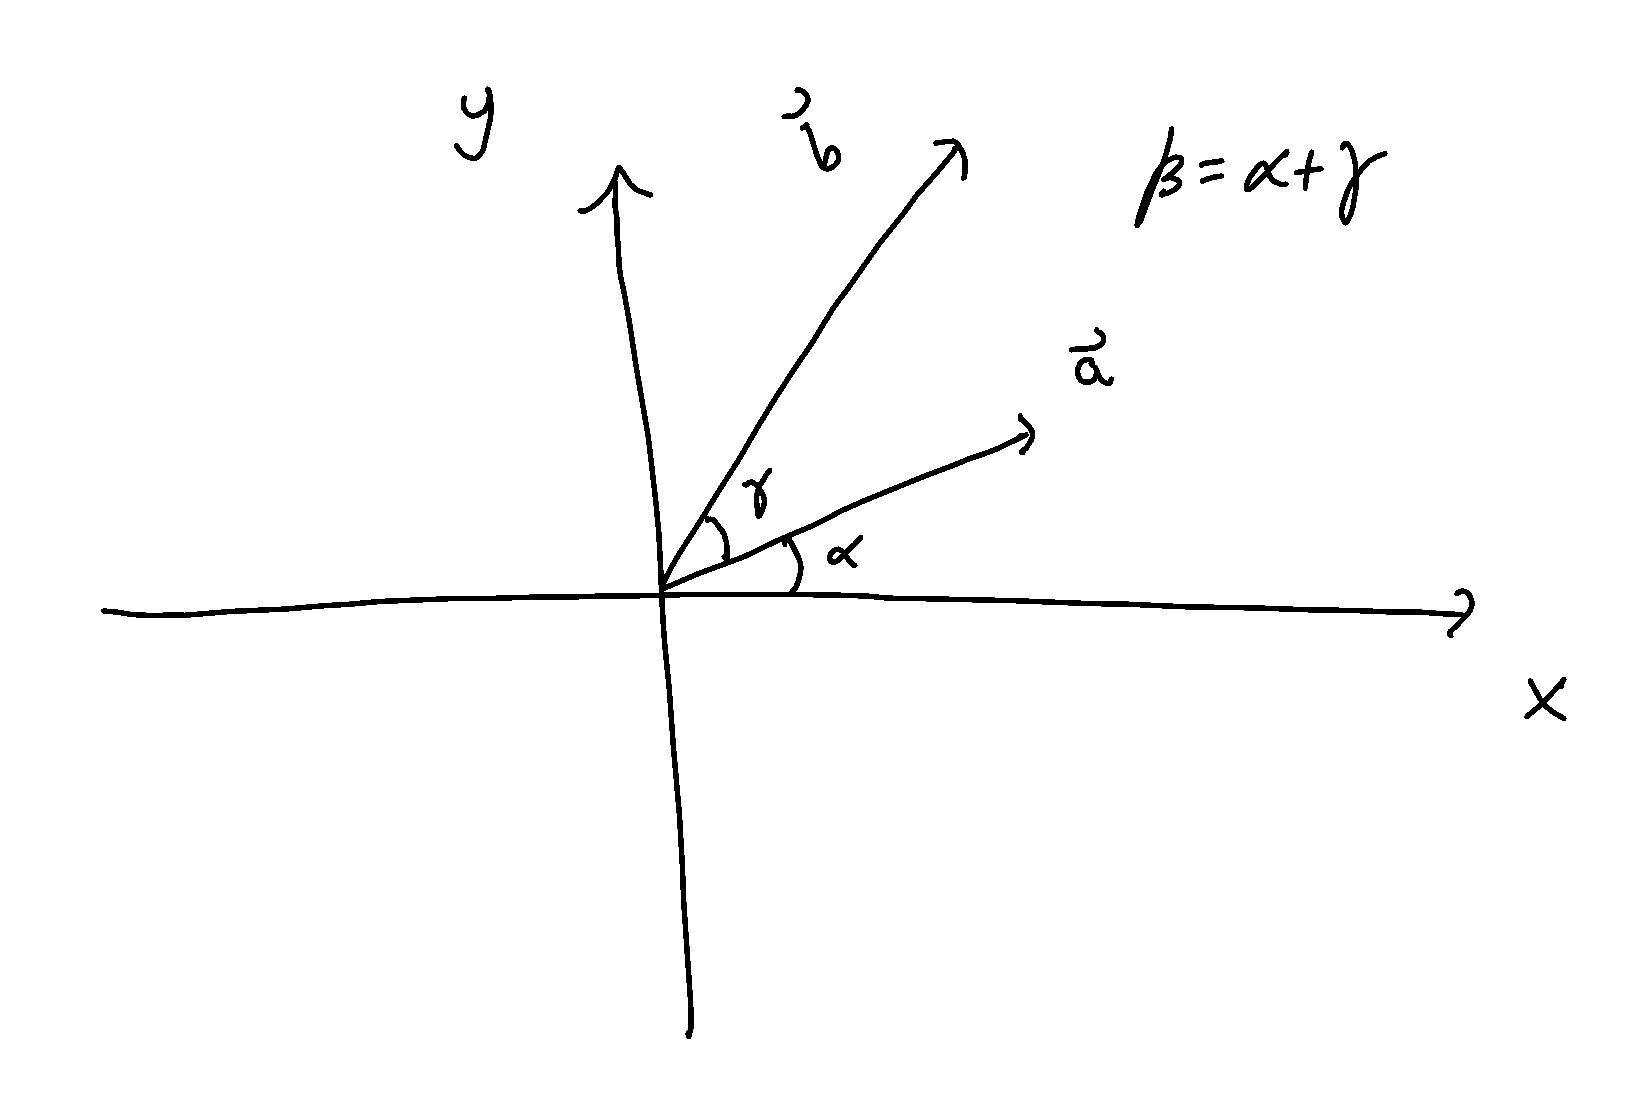
\includegraphics[width=2.5in]{temp/vigrar.png}
\caption{Tveir vigrar, $\vec{a}, \vec{b} \in \R^2$ með stefnuhorn $\alpha$ og $\beta$ hvor um sig.}
\label{fig:ab-innfeldi}
\end{wrapfigure}


\textbf{Sönnun:} Lítum á mynd \ref{fig:ab-innfeldi}. Þar má sjá tvo vigra $\vec{a} = \smqty(a_1 \\ a_2)$ og $\vec{b} = \smqty(b_1 \\ b_2)$. Við getum umritað vigrana með stefnuhornum þeirra, $\alpha$ og $\beta = \alpha + \gamma$, með eftirfarandi hætti:
\begin{align*}
    \vec{a} = \mqty(a_1 \\ a_2) = a\mqty(\cos\alpha \\ \sin\alpha),
\end{align*}
þar sem við höfum skilgreint $a = \abs{\vec{a}} = \sqrt{(a_1)^2 + (a_2)^2}$. Eins er
\begin{align*}
    \vec{b} = \mqty(b_1 \\ b_2) = b \mqty(\cos\beta \\ \sin\beta),
\end{align*}
þar sem við höfum skilgreint $b = \abs{\vec{b}} = \sqrt{(b_1)^2 + (b_2)^2}$.
\end{minipage}


Við athugum þá að innfeldi vigranna er gefið með:
\begin{align*}
    \vec{a} \cdot \vec{b} = a_1 b_1 + a_2 b_2 = ab\left( \cos\alpha \cos\beta + \sin\alpha \sin\beta \right) = ab \cos(\alpha - \beta) = ab\cos(\beta - \alpha) = ab\cos(\gamma).
\end{align*}
Þar sem við höfum notað summureglu hornafalla, að $\cos(-x) = \cos(x)$ og loks að $\beta = \alpha + \gamma$ svo $\gamma = \beta - \alpha$. \qed

\newpage

Við höfum því sýnt að við getum umritað skilgreininguna á vinnu með eftirfarandi hætti:

\begin{tcolorbox}
\begin{theorem}
Látum $\vec{F}$ vera fastann kraft sem verkar á hlut og látum $\vec{d}$ tákna færslu hlutarins á meðan að krafturinn verkar á hlutinn. Látum $\gamma$ vera hornið á milli vigranna $\vec{F}$ og $\vec{d}$ þá höfum við að:
\begin{align*}
    \vec{F} \vdot \vec{d} = F d \cos\gamma,
\end{align*}
þar sem $F = \abs{\vec{F}}$ og $d = \abs{\vec{d}\,}$. 
\end{theorem}
\end{tcolorbox}

\begin{comment}
Við gætum hinsvegar velt fyrir okkur hvað breytist ef að krafturinn $\vec{F}$ er ekki fastur. Er hægt að skilgreina vinnu fyrir krafta sem eru ekki fastir? Það er svo sannarlega hægt að skilgreina vinnu fyrir krafta sem eru ekki fastir. Þá gerum við það þannig að við skoðum örlítið tímabil og færslu hlutarins á því tímabili, þar er krafturinn svo gott sem fastur svo að við getum reiknað vinnuna hans á því tímabili. Síðan leggjum við saman öll þessi vinnuframlög yfir heildarfærsluna. Við munum skoða það nánar við tækifæri þegar þið hafið náð upp færni í stærðfræðigreiningu (diffrun og tegrun). En til bráðabirgða setjum við fram eftirfarandi:
\end{comment}

Við gætum velt fyrir okkur hvað breytist ef að krafturinn $\vec{F}$ er ekki fastur. Er hægt að skilgreina vinnu fyrir krafta sem eru ekki fastir? Það kemur í ljós að það er vissulega hægt en það þarfnast stærðfræðigreiningu (diffrun og tegrun) svo við sleppum því í bili. Niðurstaðan er hinsvegar eftirfarandi:

\begin{tcolorbox}
\begin{theorem} \label{theorem:flatarmalWork}
Látum $\Vec{F}$ vera kraft sem breytist með staðsetningu hlutarins, $\vec{s}$. Þá er vinna kraftsins, $\vec{F}$, undir færslunni $\vec{d}$, $W_F$, jöfn flatarmálinu undir krafta-stöðu grafinu.
\end{theorem}
\end{tcolorbox}

\section{Geymnir og ógeymnir kraftar}

Til þess að geta talað formlega um orku þá þurfum við að flokka kraftana sem að við höfum kynnst. Við höfum áður séð að sumir kraftar eins og t.d.~þyngdarkrafturinn varðveita orku á meðan aðrir kraftar eins og t.d.~núningskrafturinn tapa orku. Við viljum skilja hvers vegna sumir kraftar varðveita orku en aðrir ekki.

\begin{tcolorbox}
\begin{definition}
Látum $A$ og $B$ tákna tvær staðsetningar. Við segjum að kraftur, $F$, sé \textbf{geyminn} ef að heildarvinnan, $W_F$, við það að flytja hlut frá $A$ til $B$ og aftur til baka í $A$ er núll.
\end{definition}
\end{tcolorbox}

\begin{tcolorbox}
\begin{definition}
Ef krafturinn $F$ er ekki geyminn þá segjum við að hann sé \textbf{ógeyminn}.
\end{definition}
\end{tcolorbox}

Við hugsum um þetta þannig að kraftar sem eru geymnir, eins og t.d. þyngdarkrafturinn og gormkrafturinn, varðveita orku en kraftar sem eru ógeymnir eins og t.d. núningskrafturinn og loftmótsstaða, tapa orku.

\begin{tcolorbox}
\begin{theorem}
Þyngdarkrafturinn er geyminn.
\end{theorem}
\end{tcolorbox}

\begin{minipage}{\linewidth}
\begin{wrapfigure}{r}{1.5in}
\vspace{-0.5cm}
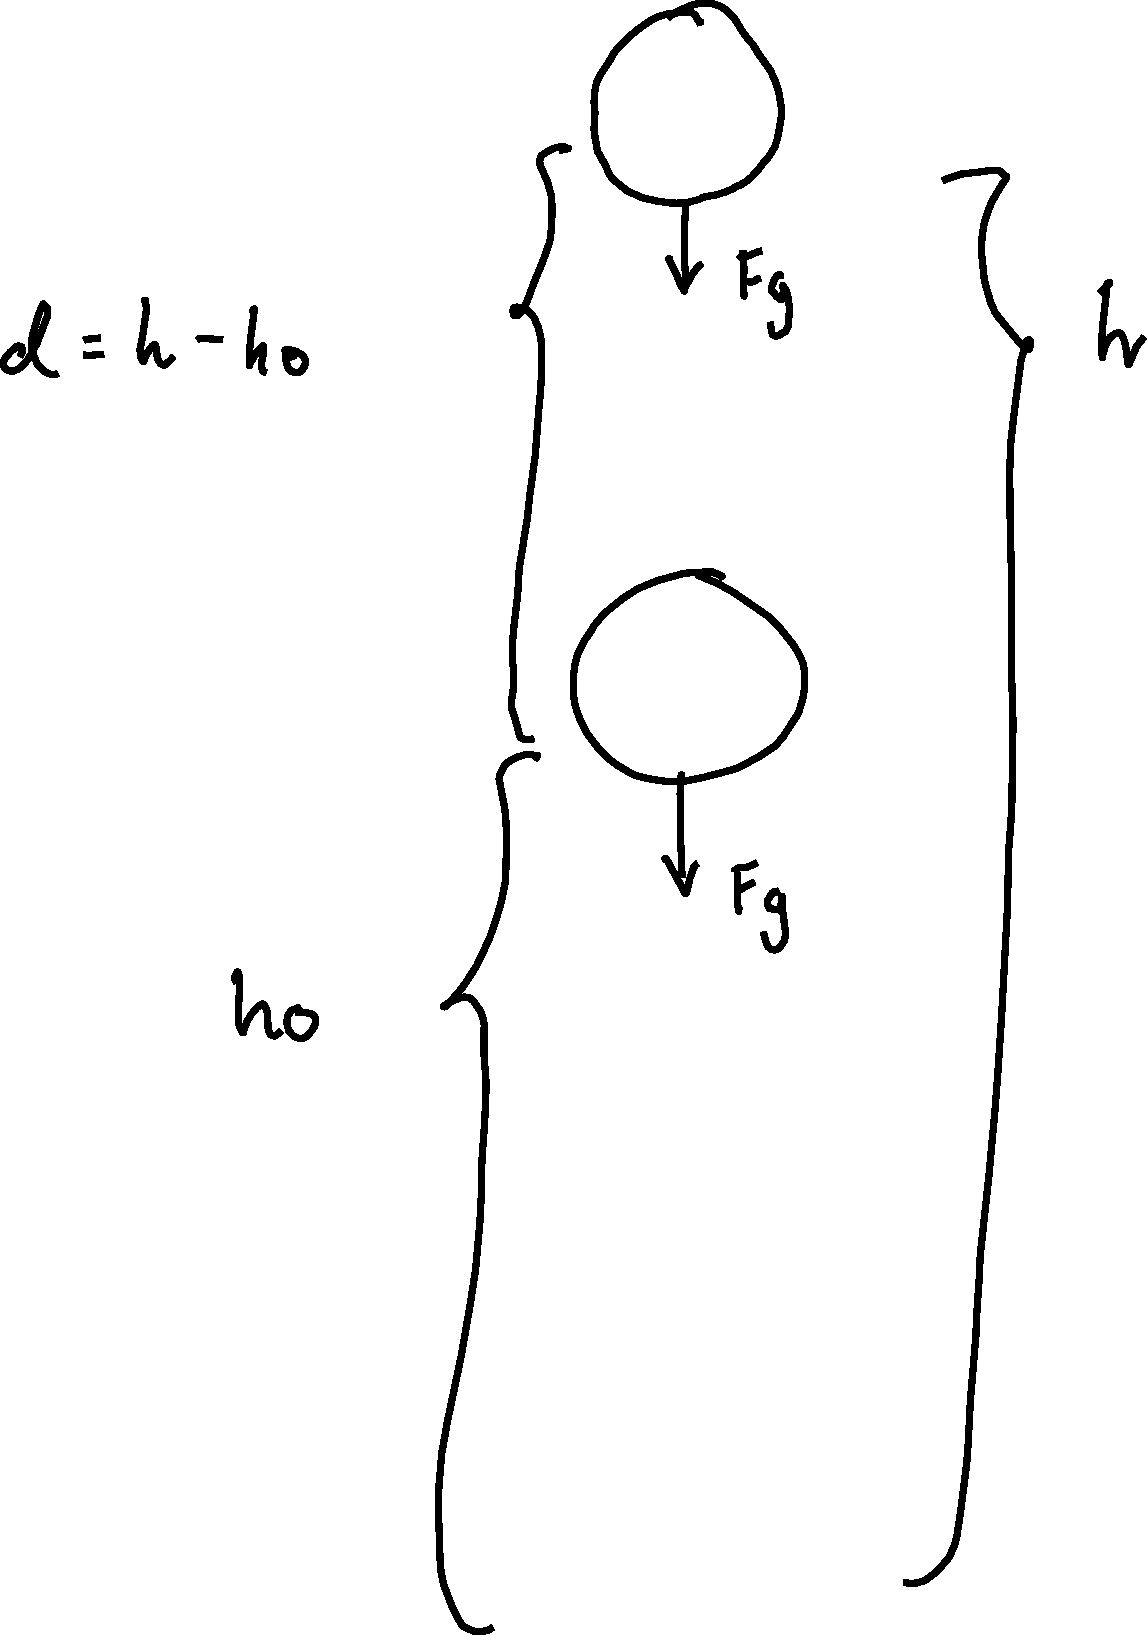
\includegraphics[width=1.5in]{temp/gravwork.pdf}
\end{wrapfigure}

\textbf{Útleiðsla:} Hugsum okkur að við köstum bolta upp í loftið. Við byrjum á því að skoða vinnu þyngdarkraftsins frá því að fara úr hæð $h_0$ upp í hæð $h$, en þá er færsla boltans $d = h-h_0$ í stefnuna upp svo að honrið á milli færslunnar og þyngdarkraftsins er $\gamma = \ang{180}$. Við fáum því að vinna þyngdarkraftsins á leiðinni upp er gefin með:
\begin{align*}
    W_g = F_g d \cos\gamma = mgd \cos(\ang{180}) = -mgd.
\end{align*}
Athugum síðan að þegar boltinn fellur úr hæð $h$ niður aftur í hæð $h_0$ þá eru þyngdarkrafturinn og færslan í sömu stefnu svo að þá er $\gamma = \ang{0}$ en þar með verður vinna þyngdarkraftsins á leiðini niður gefin með:
\begin{align*}
    W_g = F_g d \cos(\gamma) = mgd \cos(\ang{0}) = mgd.
\end{align*}
En þar með er heildarvinna þyngdarkraftsins frá því að fara úr hæð $h_0$ upp í hæð $h$ og aftur niður í $h_0$ gefin með:
\begin{align*}
    W_{\text{heild}} = -mgd + mgd = 0.
\end{align*}
\qed
\end{minipage}

\begin{tcolorbox}
\begin{theorem}
Núningskrafturinn er ógeyminn.
\end{theorem}
\end{tcolorbox}


\textbf{Útleiðsla:} Hugsum okkur að við séum að flytja kassa með massa $m$ um vegalengd $d$ meðfram gólfi og látum núningsstuðulinn milli gólfsins og kassans vera $\mu$. Þá er núningskrafturinn sem verkar á kassann gefinn með $F_{\text{nún}} = \mu mg$ í stefnuna gagnstætt hreyfingu kassans. Við höfum því að vinnan sem við vinnum við það að flytja kassann er gefin með:
\begin{align*}
    W_\mu = F_{\text{nún}} d \cos\gamma = \mu mg d \cos(\ang{180}) = -\mu mg d
\end{align*}
Þar sem að hornið á milli $\vec{F}_{\text{nún}}$ og $\vec{d}$ er $\ang{180}$.

\begin{figure}[H]
    \centering
\begin{subfigure}[h]{.45\textwidth}
    \centering
    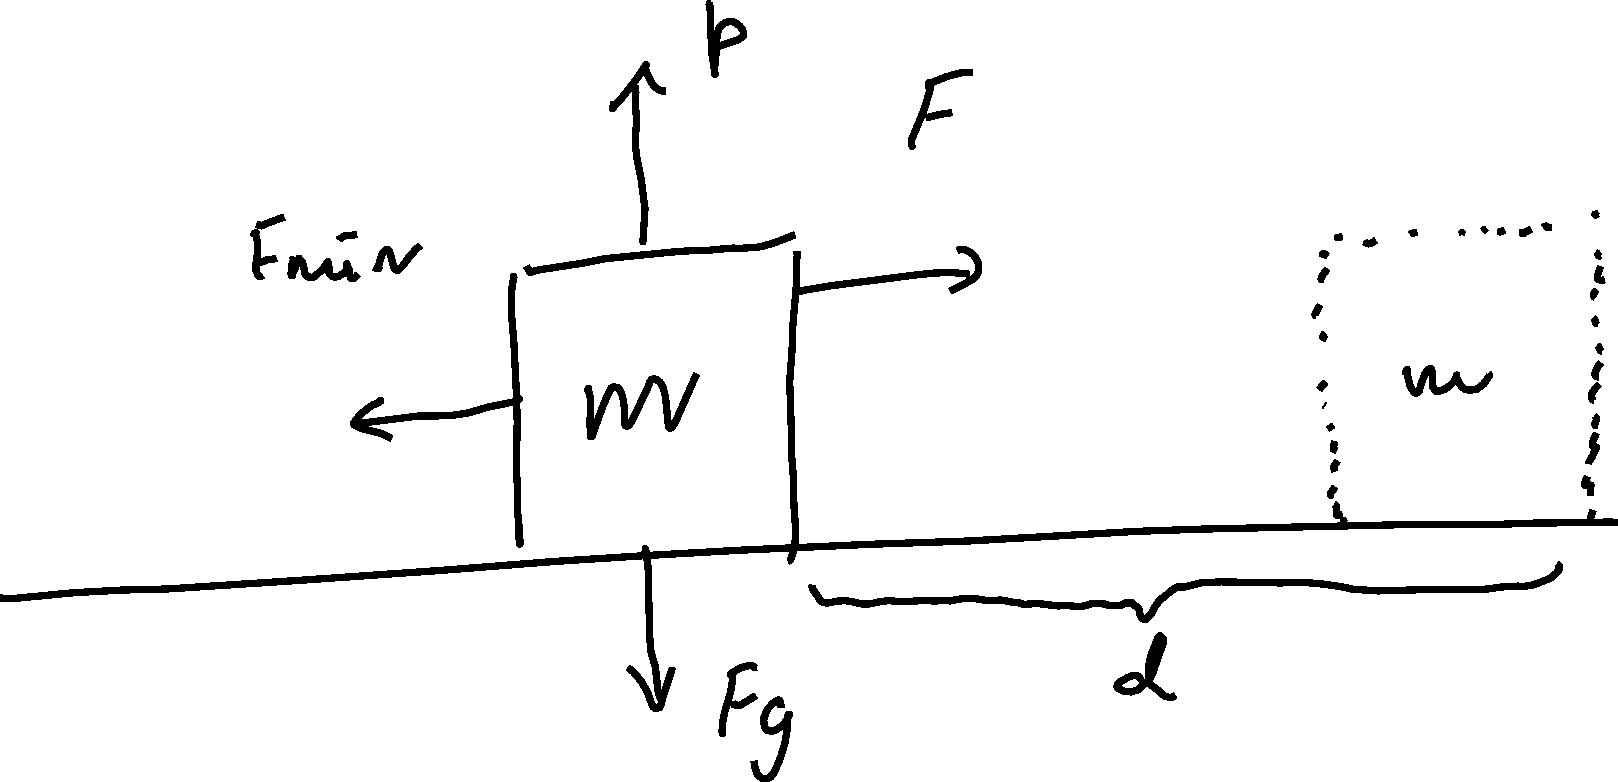
\includegraphics[width=\linewidth]{temp/worknun2.pdf}
    \caption{Kraftamynd af því að ýta kassa til hægri.}
    \label{fig:nunright}
\end{subfigure}
\hfill
\begin{subfigure}[h]{.45\textwidth}
    \centering
    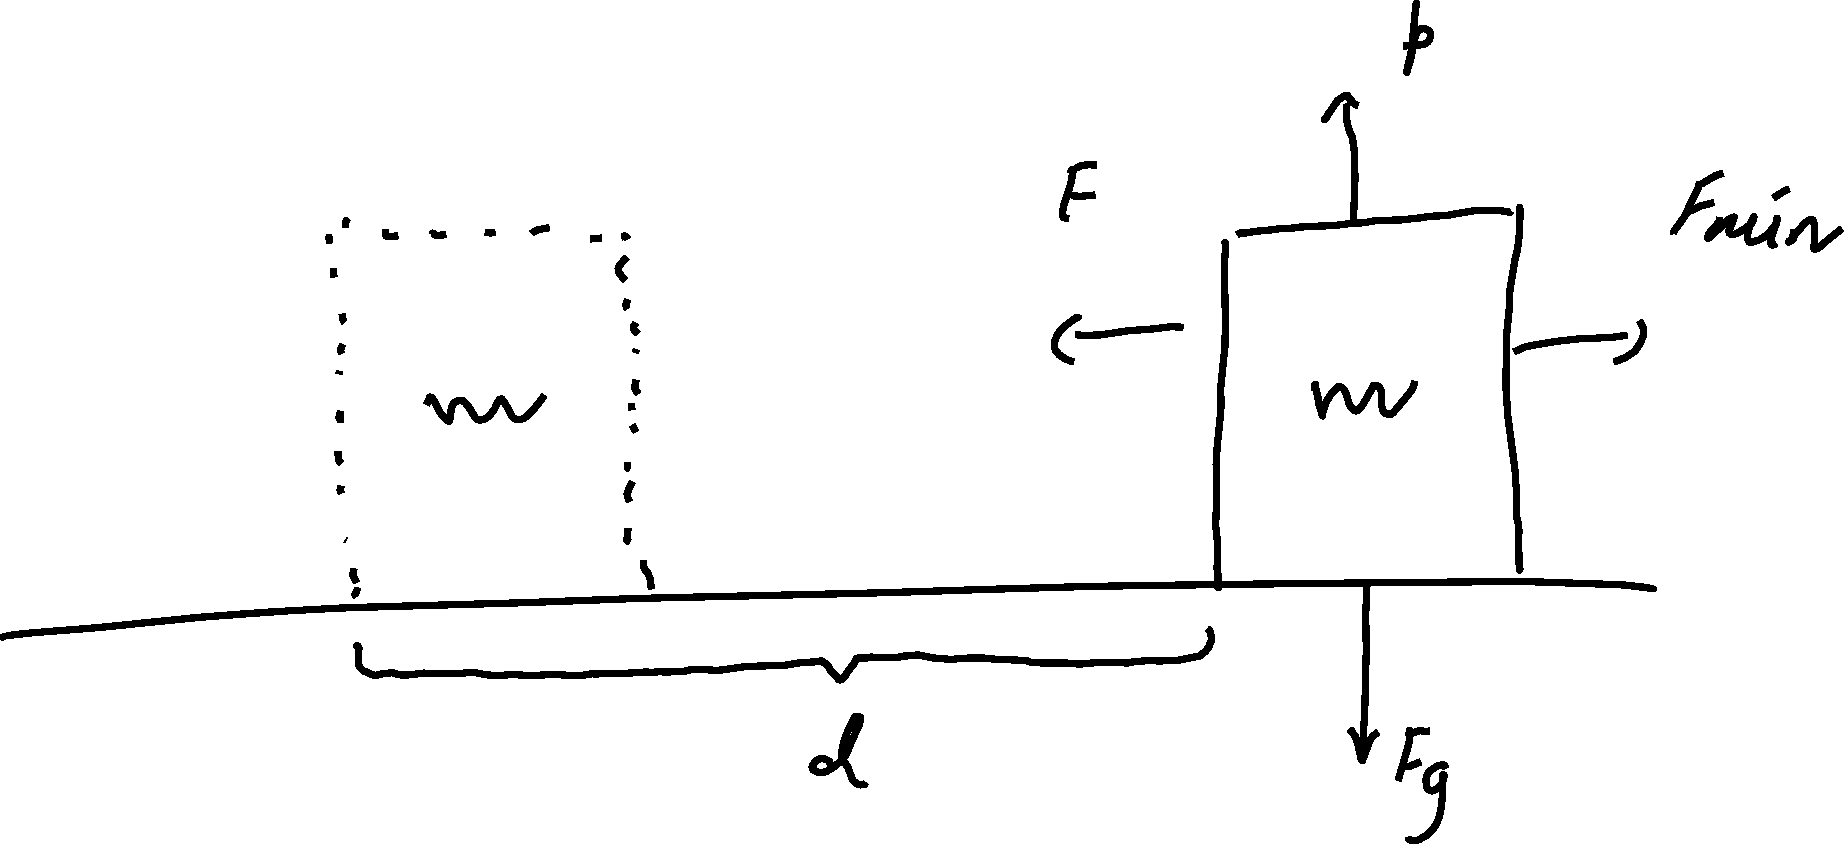
\includegraphics[width=\linewidth]{temp/worknun.pdf}
    \caption{Kraftamynd af því að ýta kassa til vinstri.}
    \label{fig:nunleft}
\end{subfigure}
\caption{Hér sést hvernig stefna núningskraftsins breytist eftir því í hvaða átt við ýtum kassanum.}
\end{figure}

Hugsum okkur nú að við ýtum kassanum til baka á staðinn þar sem hann var upphaflega staddur. Þá er núningskrafturinn aftur $F_{\text{nún}} = \mu mg$ en núna í gagnstæða stefnu miðað við áður og færsla hlutarins breytir líka um stefnu en vegalengdin er sú sama, $d$. Við ályktum því að vinna núningskraftsins við það að flytja kassann til baka er gefin með:
\begin{align*}
    W_\mu = F_{\text{nún}} d \cos\gamma = \mu mg d \cos(\ang{180}) = -\mu mg d
\end{align*}
Þar sem að hornið á milli $\vec{F}_{\text{nún}}$ og $\vec{d}$ er enn þá $\ang{180}$. Við ályktum að heildarvinna núningskraftsins við það að flytja kassann svona fram og til baka er gefin með:
\begin{align*}
    W_{\text{heild}} = -\mu mgd  - \mu mgd = -2\mu mgd \neq 0.
\end{align*}
En þar með höfum við sýnt að núningskrafturinn er ekki geyminn og þar með ógeyminn. \qed

\begin{tcolorbox}
\begin{theorem}
Gormkrafturinn er geyminn.
\end{theorem}
\end{tcolorbox}

\textbf{Útleiðsla:} Þetta þarfnast stærðfræðigreiningar (diffrun og tegrun) og því sleppum við þessu í bili.


\section{Stöðuorka}

Við erum þá loksins tilbúin til þess að skilgreina stöðuorku út frá vinnu geymins krafts:

\begin{tcolorbox}
\begin{definition}
Látum $\Vec{F}$ vera geyminn kraft. Látum $A$ og $B$ vera tvær staðsetningar. Látum $W_F$ tákna vinnu kraftsins $\vec{F}$ frá $A$ til $B$. Við skilgreinum þá stöðuorku kraftsins, $U_F$, miðað við punktinn $A$ sem stærðina:
\begin{align*}
    U_F = -W_F.
\end{align*}
\end{definition}
\end{tcolorbox}
Takið eftir að stöðuorkan er miðuð við einhvern viðmiðunarpunkt. Fyrir fasta krafta (eins og t.d.~þyngdarkraftinn) skiptir litlu máli hvar við veljum viðmiðunarpunktinn. Fyrir þyngdarkraftinn þá veljum við gjarnan jörðina sem núllpunkt hæðarinnar en við getum allt eins valið núllpunktinn uppi á Everesttindi eða ofaní Maríanadjúpálnum. Hinsvegar, fyrir krafta sem eru ekki fastir (einst og t.d.~gormkrafturinn) er þægilegast að velja viðmiðunarpunkt þar sem að krafturinn er núll.

\begin{tcolorbox}
\begin{theorem}
Stöðuorka þyngdarkraftsins, $F_g$, er gefin með:
\begin{align*}
    U_g = mgh,
\end{align*}
þar sem að $h$ táknar hæðina fyrir ofan viðmiðunarpunktinn.
\end{theorem}
\end{tcolorbox}

\textbf{Útleiðsla:} Við athugum að $\vec{F}_g$ og $\vec{d}$ eru gagnstefna svo við höfum að vinna þyngdarkraftsins er gefin með $W_g = -mgh$ en þar með er stöðuorkan gefin með $U_g = -W_g = mgh$.


\begin{tcolorbox}
\begin{theorem}
Stöðuorka gormkraftsins, $F_k$, er gefin með
\begin{align*}
    U_k = \frac{1}{2}kx^2,
\end{align*}
þar sem $k$ er gormstuðullinn og $x$ er fjarlægðin frá jafnvægisstöðunni (sem er viðmiðunarpunkturinn).
\end{theorem}
\end{tcolorbox}

\begin{minipage}{\linewidth}
\begin{wrapfigure}{r}{2.5in}
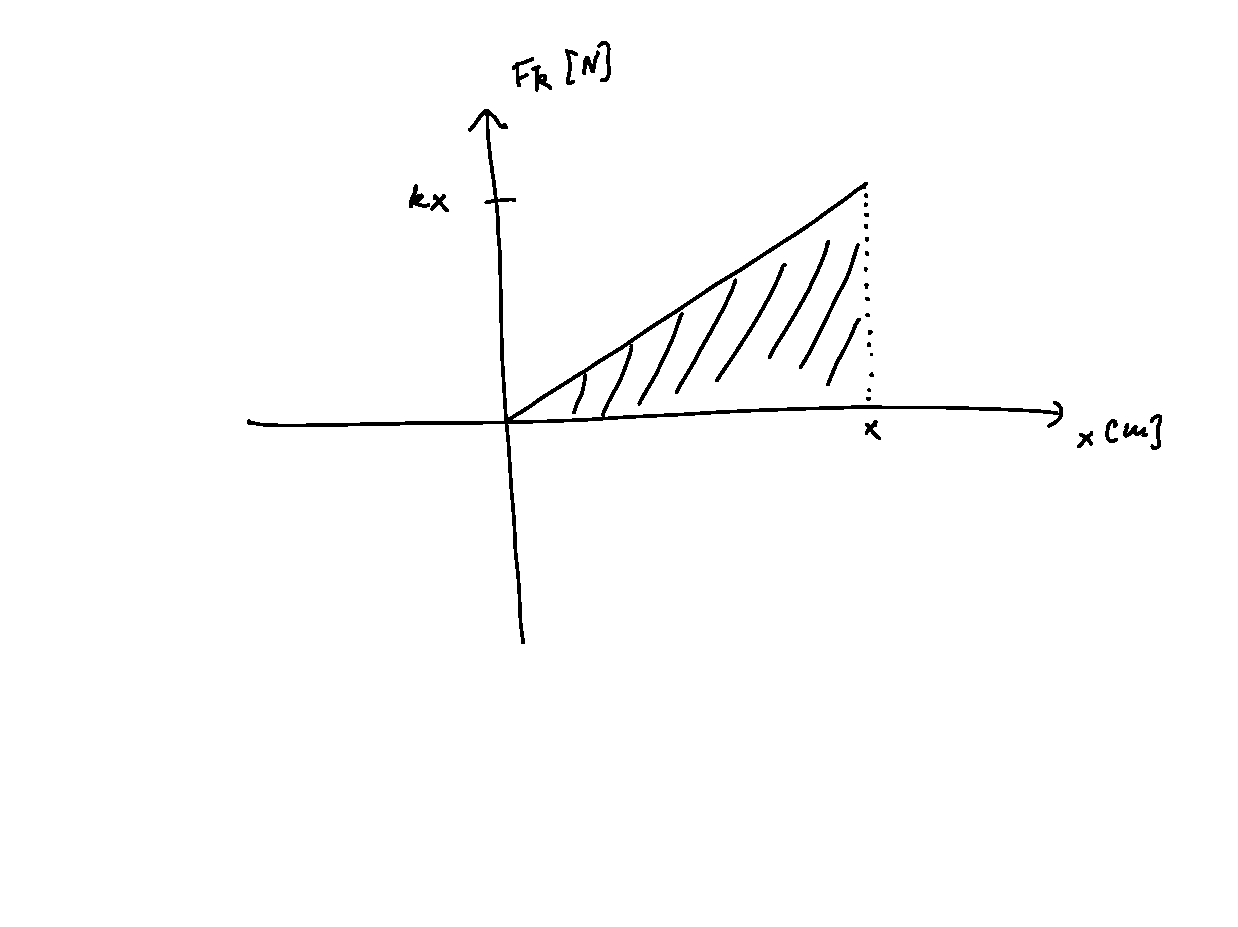
\includegraphics[width=2.5in]{temp/gormkraftur2.pdf}
\caption{$F_k = kx$ sem fall af $x$.}
\label{fig:gorm-work}
\end{wrapfigure}

\textbf{Útleiðsla:} Við nýtum okkur lögmál \ref{theorem:flatarmalWork} og skoðum graf af gormkraftinum $F_k = kx$ sem fall af $x$. Við sjáum þá að flatarmálið undir ferlinum er gefið með:
\begin{equation*}
    W_k = \frac{1}{2}(kx)x = \frac{1}{2}kx^2.
\end{equation*}
En við vitum að gormkrafturinn og færslan eru gagnstefna svo að við höfum að $W_k = -\frac{1}{2}kx^2$ (Grafið sem við teiknuðum hér til hægri ætti í rauninni að skipta út fyrir graf af $F_k = -kx$ sem fall af $x$). En þar með getum við ályktað að stöðuorka gormkraftsins miðað við jafnvægisstöðuna er gefin með:
\begin{equation*}
    U_k = -W_k = \frac{1}{2}kx^2.
\end{equation*}

\end{minipage}

\section{Orkuvarðveisla}


\begin{tcolorbox}
\begin{theorem}
\textbf{(Vinnulögmálið)} Látum $E_1$ tákna heildarorku hlutar við tíma $t_1$ og látum $E_2$ tákna heildarorku hlutar við tíma $t_2 > t_1$. Látum $W$ tákna vinnu ógeyminna krafta á þessum tíma. Þá er:
\begin{align*}
    E_1 + W = E_2.
\end{align*}
\end{theorem}
\end{tcolorbox}


\textbf{Útleiðsla:} Við sjáum nú að ef á hlut verkar kraftur $F_{\text{heild}}$ þá er vinnan:
\begin{equation*}
    W_{\text{heild}} = \vec{F}_{\text{heild}} \cdot \Delta \vec{s} = m \vec{a} \cdot \Delta \vec{s} = m \frac{v_2^2 - v_1^2}{2} = \Delta K.
\end{equation*}
Við skulum nú skipta vinnu kraftanna sem verka á hlutinn upp í vinnu geyminna krafta, $W_\text{g}$ og ógeyminna krafta $W_\mu$. Þá er $\Delta K = W_{\text{heild}} = W_g + W_\mu$ og við höfum að:
\begin{equation*}
    \Delta E = \Delta K + \Delta U = \Delta K - W_g = \Delta K - (W_g + W_\mu - W_\mu) =  \Delta K - W_{\text{heild}} + W_\mu = W_\mu
\end{equation*}
En þar með höfum við einmitt sýnt að $E_1 + W_\mu = E_2$. \qed

\begin{tcolorbox}
\begin{theorem}
Ef engir ógeymnir kraftar verka á hlut þá er heildarorka hlutarins varðveitt.
\end{theorem}
\end{tcolorbox}

\newpage

\section{Skriðþungavarðveisla}

Við höfum enn ekki talað um tengsl skriðþunga, $p = mv$, við krafta, $F = ma$. Það er nefnilega til önnur leið til þess að skilgreina kraft. Við athugum að $a = \frac{dv}{dt}$ svo við höfum að:
\begin{align*}
    F = ma = m\frac{dv}{dt} = \frac{d(mv)}{dt} = \frac{dp}{dt}.
\end{align*}
En þetta segir okkur að kraftur er það sama og breyting í skriðþunga, $dp$, á tíma $dt$. Við sjáum því að:

\begin{tcolorbox}
\begin{theorem}
Ef enginn heildarkraftur verkar á hlut þá er skriðþungi hlutarins varðveittur.
\end{theorem}
\end{tcolorbox}

\textbf{Útleiðsla:} Við sjáum að ef $F = 0$ þá er $\frac{dp}{dt} = 0$ en það þýðir að skriðþungi hlutarins er ekki að breytast með tíma svo skriðþunginn er varðveittur. \qed

\begin{tcolorbox}
\begin{theorem}
Lítum á hlut með massa $m_1$ og hraða $v_1$ og hlut með massa $m_2$ og hraða $v_2$ sem lenda í árekstri. Þá er heildarskriðþunginn, $p_{\text{heild}} = m_1 v_1 + m_2 v_2$ varðveittur í árekstrum.
\end{theorem}
\end{tcolorbox}

\textbf{Útleiðsla:} Í árekstrinum þá er eini krafturinn sem verkar á milli hlutanna, þriðja lögmáls gagnkrafturinn á milli hlutanna svo við höfum að:
\begin{align*}
    F_{1} = -F_{2} \implies \frac{dp_1}{dt} = -\frac{dp_2}{dt} \implies \frac{d}{dt}\left( p_1 + p_2 \right) = 0 \implies \explain{p_1 + p_2}{p_{\text{heild}}} = \text{fasti}.
\end{align*}
\qed

\section{Sýnidæmi}


\begin{minipage}{\linewidth}
\begin{wrapfigure}{r}{2.8in}
\vspace{-1cm}
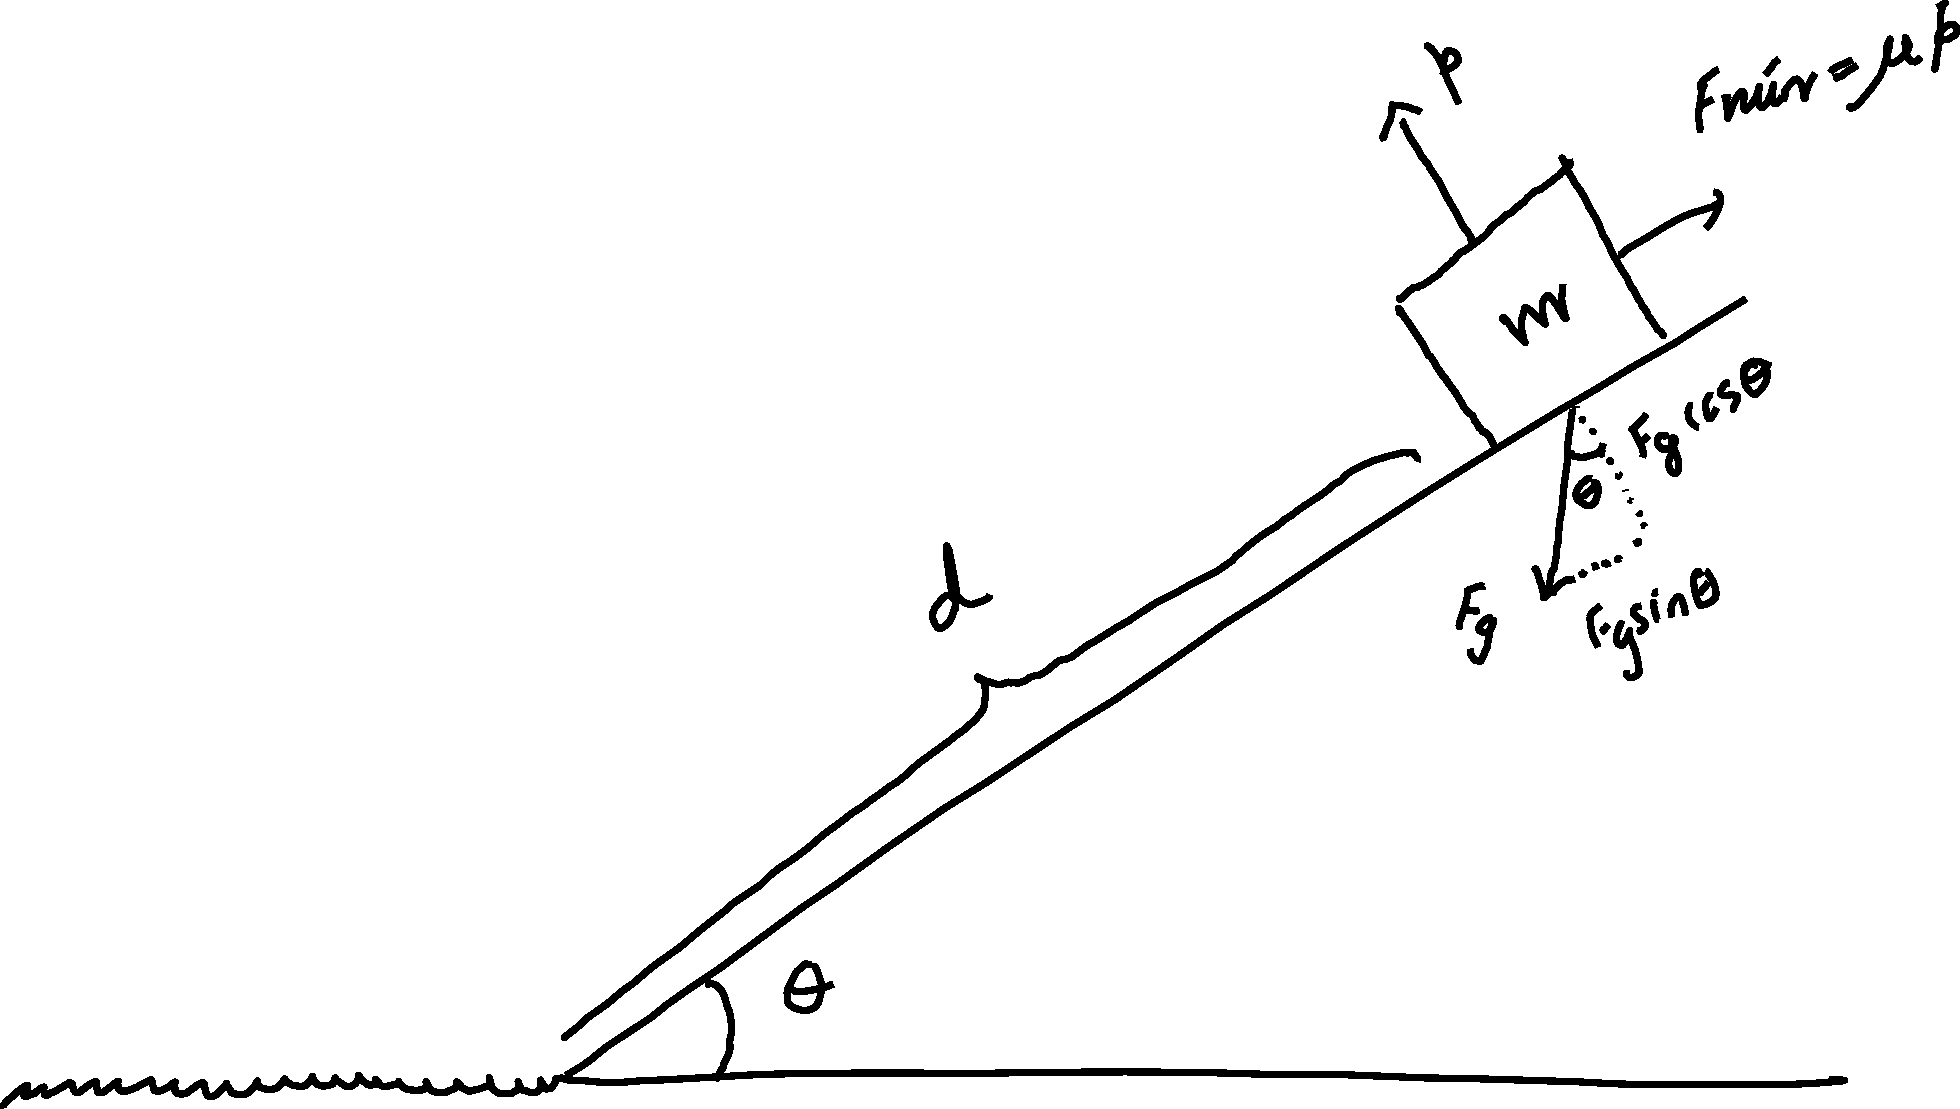
\includegraphics[width=3in]{temp/fnun.pdf}
\caption{Hlutur að renna niður skábretti.}
\label{fig:fnun}
\end{wrapfigure}

Lítum á kassa með massa $m$ sem byrjar í hæð $h$ á skábretti sem hallar um horn $\theta$ miðað við lárétt. Núningsstuðullinn milli skábrettisins og kassans er $\mu_s$. Eftir að kassinn hefur runnið niður tekur við hrjúft yfirborð þar sem núningsstuðullinn milli kassans og yfirborðsins er $\mu_h$. Við viljum ákvarða vegalengdina $x$ sem kassinn mun renna meðfram hrjúfa yfirborðinu áður en hann stöðvast. Við byrjum því á því að athuga að vegalengdin $d$ sem að kassinn mun renna niður skábrettið er gefin með $d = \frac{h}{\sin\theta}$. Við höfum síðan eftirfarandi kraftajöfnu fyrir kassann þegar hann er í efstu hæð:
\begin{align*}
    \mqty(ma \\ 0) = \mqty(mg\sin\theta - F_{\text{nún}} \\ Þ - mg\cos\theta)
\end{align*}
Sem gefur því að $F_{\text{nún}} = \mu_s Þ = \mu_s mg\cos\theta$. Vinna núningskraftsins á leiðnni niður skábrettið er því gefin með: $W_{\mu_s} = -\mu_s mgd\cos\theta$ þar sem að $\vec{d}$ og $\vec{F}_{\text{nún}}$ eru gagnstefna. Við höfum samkvæmt vinnulögmálinu að:
\begin{align*}
    mgh - \mu_s mgd\cos\theta = \frac{1}{2}mv^2 \implies v = \sqrt{2\left(gh - \mu_s gd \cos\theta \right)} = \sqrt{2gh\left(1 - \mu_s \cot\theta \right)}
\end{align*}
Þar sem $v$ er hraði kassans þegar hann kemur niður skábrettið. En síðan vitum við að þar tekur við nýtt yfirborð þar sem að þverkrafturinn er $Þ = mg$ og núningskrafturinn verður $F_{\text{nún}} = \mu_h Þ = \mu_h mg$ og vinna núningskraftsins þar til hann stöðvast er gefin með $W_{\mu_h} = -\mu_h mgx$ svo við höfum að:
\begin{align*}
    \frac{1}{2}mv^2 - \mu_h mgx = 0 \implies x = \frac{1}{\mu_h}\left(1- \mu_s \cot\theta \right)h.
\end{align*}


\end{minipage}






\newpage


\section{Dæmi}

\begin{enumerate}[label = \textbf{Dæmi \thechapter.\arabic*.}]


\subsection*{Vinna}

\begin{minipage}{\linewidth}
\begin{wrapfigure}{r}{1.1in}
\vspace{-0.5cm}
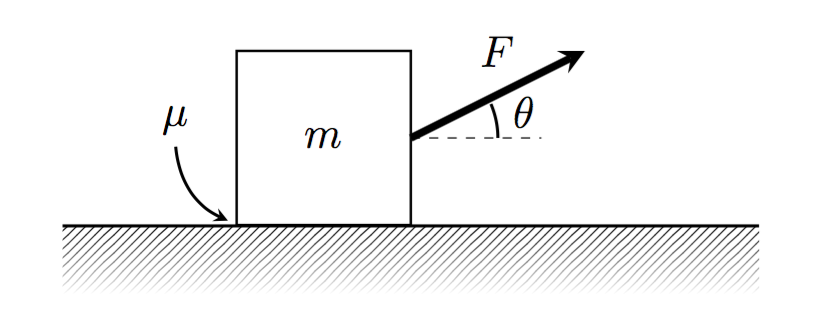
\includegraphics[width=1.7in]{images/beggatwerk.png}
\end{wrapfigure}
    
    \item Bergljót er að færa stóra, þunga eldavél með massa $m = \SI{120}{kg}$ í íbúðinni sinni. Núningsstuðullinn milli eldavélarinnar og gólfsins er $\mu = 0,40$. Nauðsynlegt er að draga eldavélina með jöfnum hraða svo hún springi ekki. Bergljót dregur eldavélina með krafti $F$ undir horninu $\theta = \SI{31}{\degree}$. Hversu mikla vinnu vinnur Bergljót við það að flytja eldavélina um $\SI{8,4}{m}$ að því gefnu að eldavélin springi ekki?
    
\end{minipage}
    
\begin{minipage}{\linewidth}
\begin{wrapfigure}{r}{1.1in}
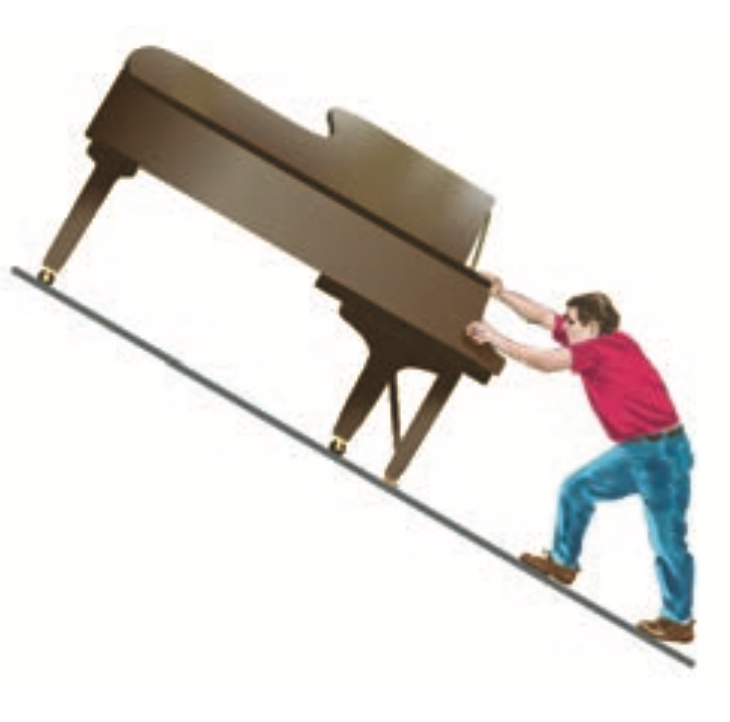
\includegraphics[width=1.2in]{images/pianoman.png}
\end{wrapfigure}
    
    \item Píanó sem hefur massa $m = \SI{380}{kg}$ rennur  niður $\SI{2.9}{m}$ langa brekku sem hallar um $\theta = \ang{25}$ miðað við lárétt. Núningsstuðullinn milli skábrettisins og píanósins er $\mu = 0.18$. Sigbert sterkbygði heldur í við píanóið með því að ýta á það með krafti samsíða skábrettinu. Hann passar að píanóið renni niður með jöfnum hraða.
    
\end{minipage}
    
    \begin{enumerate}[label = \textbf{(\alph*)}]
        \item Hver er stærð kraftsins sem að Sigbert ýtir með á píanóið?
        
        \item Hversu mikla vinnu vinnur Sigbert á píanóið á leiðinni niður brekkuna?
        
        \item Hversu mikla vinnu vinnur þyngdarkrafturinn á píanóið á leiðinni niður brekkuna?
        
        \item Hversu mikla vinnu vinnur núningskrafturinn á píanóið á leiðinni niður brekkuna?
        
        \item Hversu mikla vinnu vinnur þverkrafturinn á píanóið á leiðinni niður brekkuna?
        
        \item Hver er vinna heildarkraftsins sem verkar á píanóið á leiðinni niður brekkuna? 
    \end{enumerate}

    
\begin{minipage}{\linewidth}
\begin{wrapfigure}{r}{2in}
\vspace{-0.75cm}
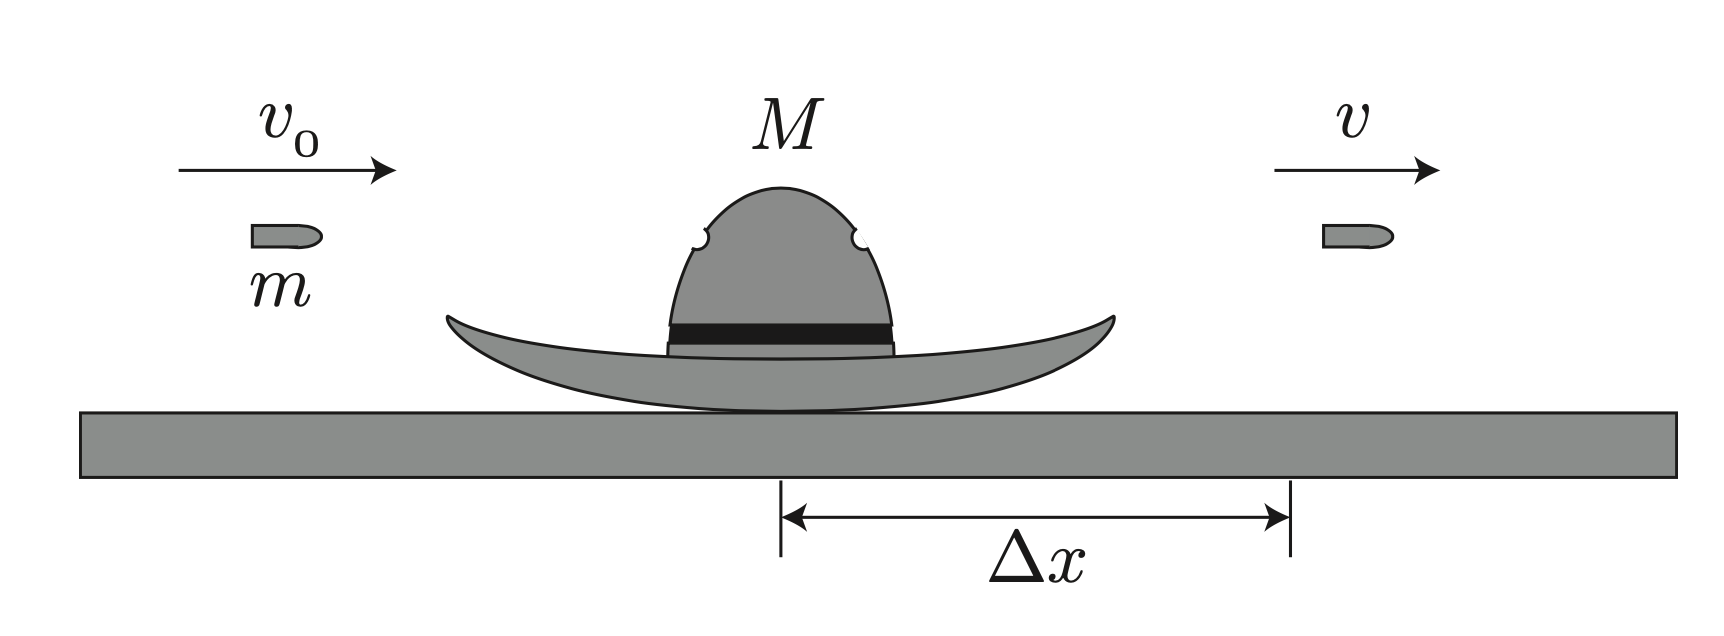
\includegraphics[width=2.25in]{images/hattur.png}
\end{wrapfigure}

    \item Kúrekahattur með massa $M = \SI{130}{g}$ hvílir á borði. Núningsstuðullinn milli hattsins og borðsins er $\mu = 0.25$. Byssukúlu með massa $m = \SI{5}{g}$ og láréttan hraða $v_0 = \SI{550}{m/s}$ er skotið í gegnum kúrekahattinn þannig að hann rennur $\Delta x = \SI{1.25}{m}$ eftir borðinu. Hver er hraði byssukúlunnar, $v$, eftir að hún kemur út úr hattinum?
    
\end{minipage}
    
\begin{minipage}{\linewidth}
\begin{wrapfigure}{r}{2in}
\vspace{-1cm}
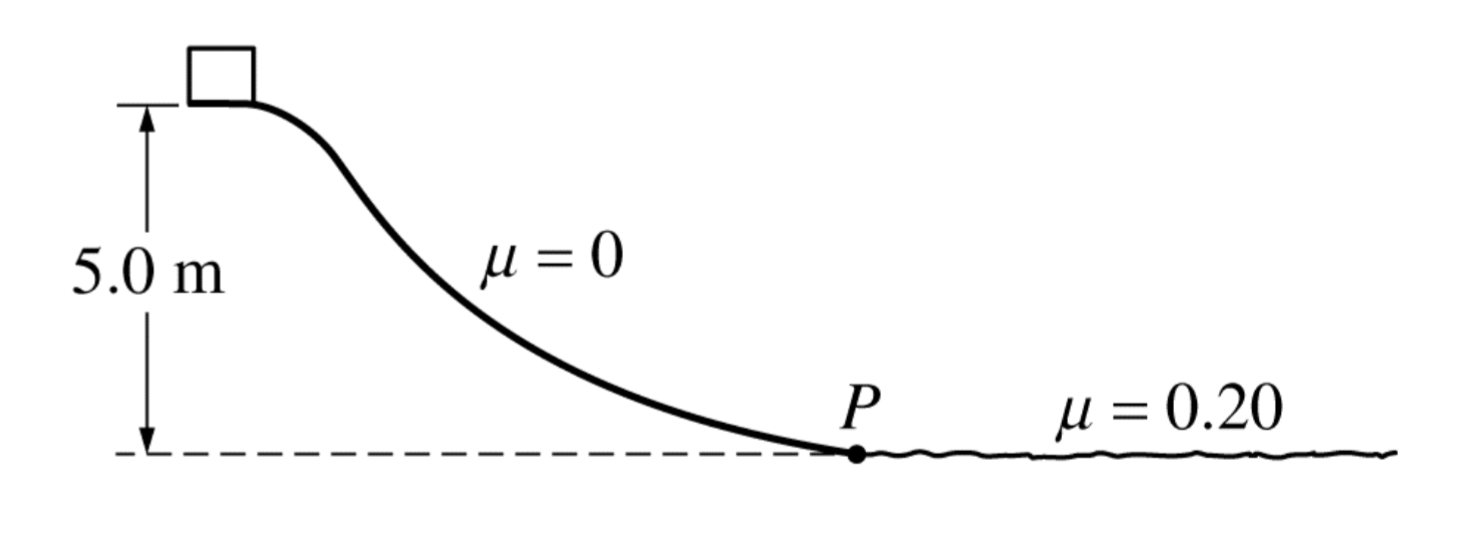
\includegraphics[width=2.25in]{images/nun.png}
\end{wrapfigure}

    \item Kubbur með massa $\SI{3.0}{kg}$ rennur úr kyrrstöðu niður brekku með hverfandi núning úr hæðinni $\SI{5.0}{m}$. Eftir að kubburinn hefur runnið framhjá punkti $P$ tekur við hrjúft, lárétt yfirborð þar sem núningsstuðullinn milli kubbsins og yfirborðsins er $0.20$. Hversu langt rennur kubburinn eftir lárétta yfirborðinu áður en hann stöðvast?

\end{minipage}

\item Hugsum okkur að við séum að ýta bíl með massa $m = \SI{950}{kg}$ upp $\SI{710}{m}$ langa brekku sem hallar um $\theta = \ang{12}$ miðað við lárétt. Núningsstuðullinn milli bíldekkjanna og malbiksins er $\mu = 0.05$. Hver er minnsta vinnan sem við þurfum að vinna til að ýta bílnum upp brekkuna?


\item Tesla Model S sportbíll með massa $m_T = \SI{2250}{kg}$ skellur harkalega aftan í kyrrstæðri, lítilli rútu með massa $m_R = \SI{3550}{kg}$ sem stöðvaði á rauðu ljósi. Bílarnir festast saman í árekstrinum og renna $\SI{6.6}{m}$ áður en þeir stöðvast. Lalli lögreglumaður er fjölkunnugur og rifjar upp eðlisfræðina sem hann lærði í menntaskóla. Hann ákveður að reikna vinnuna sem tapaðist í núning til þess að finna hraða Teslunnar fyrir áreksturinn. Hann veit að núningsstuðullinn milli bíldekkja og malbiks er $\mu = 0.80$. Hver var hraði Teslunnar fyrir áreksturinn?


\item Byssukúlu með massa $m = \SI{5.0}{g}$ er skotið beint upp með hraðanum $\SI{500}{m/s}$. Byssukúlan lendir í trjágrein, fer í gegnum hana og kemur út með hraðanum $\SI{100}{m/s}$. Efri brún trjágreinarinnar er í $\SI{15}{m}$ hæð. Trjágreinin er $\SI{20}{cm}$ þykk þar sem kúlan fór í gegn. Hversu mikla vinnu framkvæmdi trjágreinin á byssukúlunni? Hver var meðalkraftur trjágreinarinnar á byssukúluna?

\item Bíll með massa $m = \SI{2000}{kg}$ ekur á hraðanum $\SI{25}{m/s}$ eftir láréttum vegi. Skyndilega verður ökumaðurinn var við kött á veginum og nauðhemlar til að reyna að bjarga kettinum. Bíllinn stöðvast eftir $\SI{60}{m}$. Metið vinnu núningskraftsins og núningsstuðulinn milli dekkjanna og vegarins.
    

\item Skíðakappi með massa $\SI{80}{kg}$ stendur efst í Kóngsgili í Bláfjöllum. Hann lætur sig renna af stað og fer beint í brunastellingu. Þegar hann kemur niður á jafnsléttu $\SI{200}{m}$ neðar er hraði hans $\SI{120}{km/klst}$. Ef engir núningskraftar hefðu verkað á skíðakappann, hver ætti þá hraði hans að hafa verið þegar hann kæmi niður? Hver er heildarvinna ógeyminna krafta á skíðakappann fyrst hraði hans var aðeins $\SI{120}{km/klst}$ þegar hann kom niður?

\subsection*{Gormar}
    
\begin{minipage}{\linewidth}
\begin{wrapfigure}{r}{1.7in}
\vspace{-1.5cm}
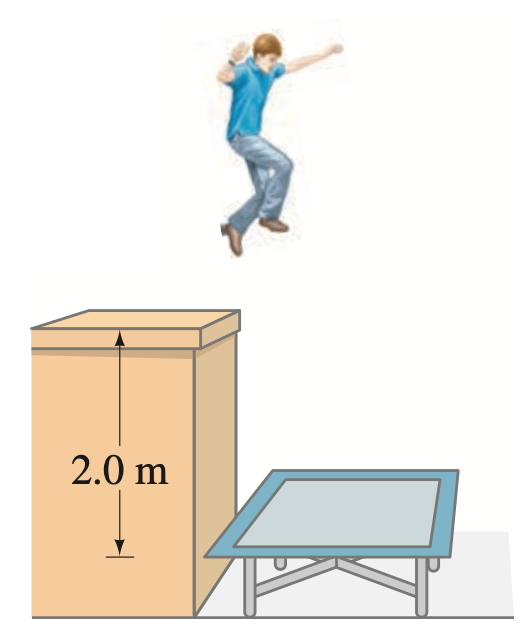
\includegraphics[width=1.7in]{images/hopp.png}
\end{wrapfigure}
    
    \item Kiddi kærulausi hefur massann $m = \SI{62}{kg}$. Hann hoppar fram af bílskúrsþakinu heima hjá sér með lóðréttum upphafshraða $v_0 = \SI{4.5}{m/s}$ og lendir á trampólíni $\SI{2.0}{m}$ fyrir neðan. 
    
    \begin{enumerate}[label = \textbf{(\alph*)}]
        \item Hver er hraði hans rétt áður en hann lendir á trampólíninu?
        
        \item Gera má þá nálgun að trampólínið hegði sér eins og gormur með gormstuðul $k = \SI{5.8e4}{N/m}$. Hversu langt mun trampólínsdúkurinn síga niður?
    \end{enumerate}
    
    \end{minipage}
    
\begin{minipage}{\linewidth}
\begin{wrapfigure}{r}{1.7in}
\vspace{1cm}
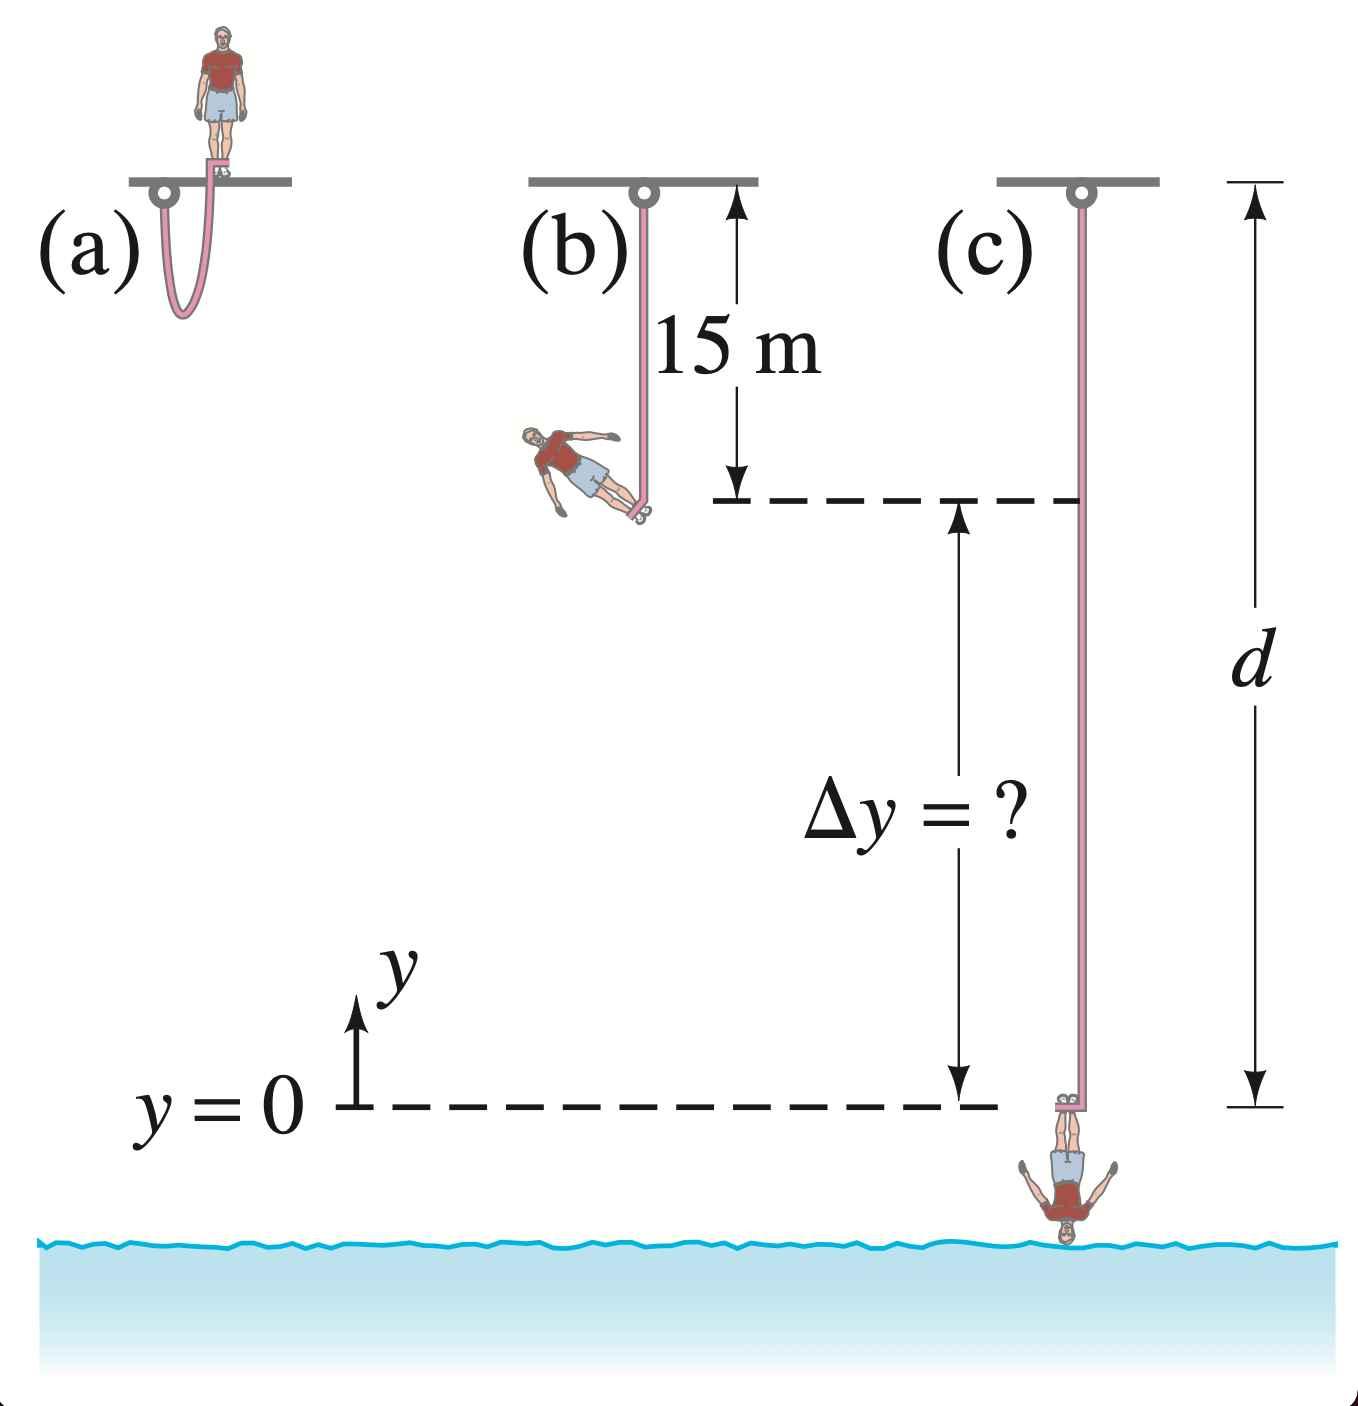
\includegraphics[width=1.7in]{kaflar/kafli07/figures/frikki.png}
%\caption*{(a) Áður en Friðrik stekkur. (b) Áður en það byrjar að strekkjast á teygjunni. (c) Mesta strekking teygjunnar.}
\end{wrapfigure}
    
    \item Friðrik fífldjarfi (með massa $m = \SI{75}{kg}$) fer í teygjustökk fram af brú. Óstrekkt lengd teygjunnar er $\ell = \SI{15}{m}$ svo hann dettur í $\SI{15}{m}$ áður en að það byrjar að togna á teygjunni. Lýsa má strekkingu teygjunnar eins og gormi með gormstuðul $k = \SI{55}{N/m}$. Ákvarðið fallvegalengdina, $d$, sem Friðrik fellur þar til hann staðnæmist um stundarkorn í lægstu stöðu og áður en hann skýst síðan aftur upp. Hunsið loftmótsstöðu og massa teygjunnar.
    
    
    \item Kubbur með massa $m_1 = \SI{4.0}{kg}$ er festur í jafnvægisstöðu við gorm með gormstuðul $k_1 = \SI{20}{N/m}$. Gormurinn er síðan þjappaður saman um lengdina $d = \SI{5.2}{cm}$. Kubburinn er þar losaður frá gorminum og síðan er honum sleppt. Hann rennur þá eftir núningslausa fletinum sem hann hvílir á þar til hann rekst á kyrrstæðan kubb með massa $m_2 = \SI{3.0}{kg}$ sem er festur við gorm með gormstuðul $k_2 = \SI{28}{N/m}$. Kubbarnir festast saman við áreksturinn.

\end{minipage}

\begin{figure}[H]
    \centering
    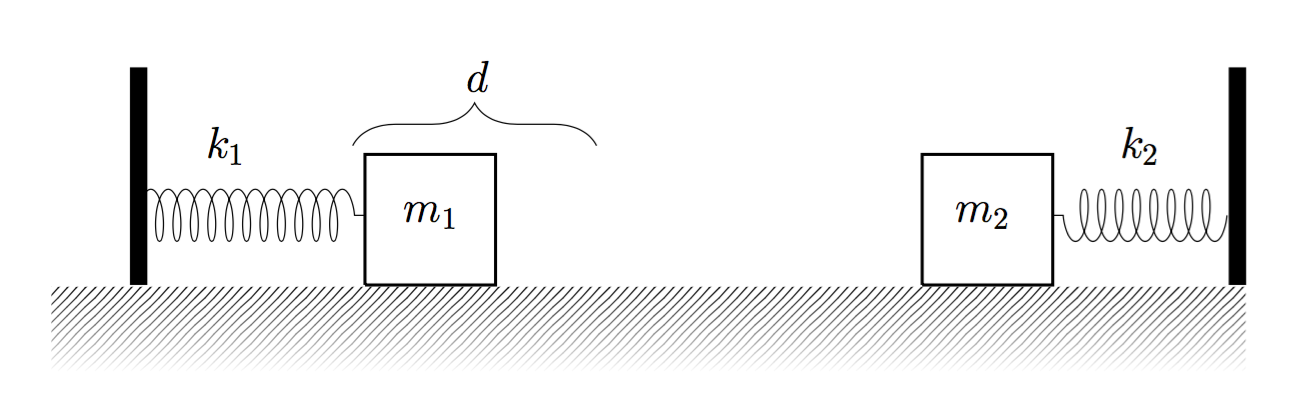
\includegraphics[scale = 0.35]{images/gormur.png}
\end{figure}

\begin{enumerate}[label = \textbf{(\alph*)}]
    \item Finnið hraða kubbsins með massa $m_1$ rétt fyrir áreksturinn.

    \item Finnið hraða kubbanna rétt eftir áreksturinn með því að nota skriðþungavarðveislu.
    
    \item Finnið mestu þjöppun gormsins eftir áreksturinn.
    
    \item Finnið orkuna sem tapast við áreksturinn.
\end{enumerate}

\begin{minipage}{\linewidth}
\begin{wrapfigure}{r}{2.3in}
\vspace{-0.5cm}
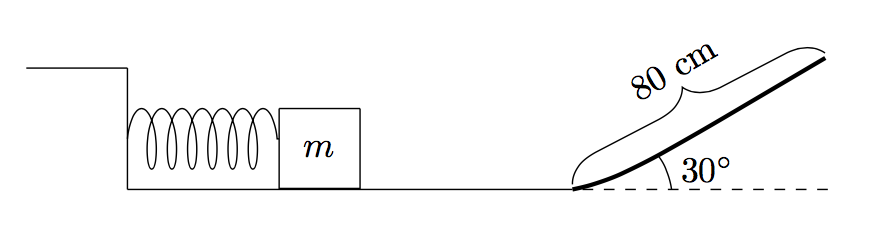
\includegraphics[width=2.5in]{images/rampurmerking.png}
\end{wrapfigure}

\item Kassa með massa $m = \SI{2.5}{kg}$ er sleppt efst á núningslausu skábretti sem hallar um $\theta = \ang{30}$ miðað við lárétt. Þar á eftir rennur kassinn meðfram núningslausu gólfi þar til hann þrýstir saman gormi sem fastur er við vegg. Hver er mesta þjöppun gormsins ef kraftstuðull gormsins er $k = \SI{400}{N/m}$?

\end{minipage}

\item Kassi með massa $m=\SI{0,1}{kg}$ situr á núningslausri braut. Honum er ýtt upp við gorm með gormstuðul $k=\SI{1,8}{N/m}$ þ.a. gormurinn sé \SI{50}{cm} frá jafnvægisstöðu. Síðan er kassanum sleppt og hann rennur eftir 80 cm löngum rampi sem myndar 30$^{\circ}$ horn við lárétt. Hve langt eftir rampinum ferðast kassinn áður en hann stoppar?

\item Gormur með gormstuðul $k = \SI{600}{N/m}$ er festur í annan endann við vegg. Við hinn endann er kassi með massa $m = \SI{6.8}{kg}$ festur. Kassinn stendur á láréttu borði og núningsstuðulinn milli borðsins og kubbsins er $\mu$. Gorminum er nú þjappað saman um $x = \SI{18}{cm}$ frá jafnvægisstöðunni sinni og sleppt. Þegar gormurinn er kominn aftur í jafnvægisstöðu sína í $x = 0$, er hraði massans $v = \SI{1.3}{m/s}$. Reiknið vinnu núningskraftsins og núningsstuðulinn milli borðs og kubbs.

\item Fær bogaskytta dregur bogastrenginn aftur um $\SI{50}{cm}$ með $\SI{150}{N}$ krafti og sleppir ör með massa $\SI{100}{g}$ af stað. Gera má ráð fyrir að krafturinn sem boginn verkar með á örina hegði sér eins og gormur með gormstuðul $k$. Hver er hraði örvarinnar um leið og hún losnar af strengnum?

\begin{minipage}{\linewidth}
\begin{wrapfigure}{r}{1.7in}
\vspace{-0.75cm}
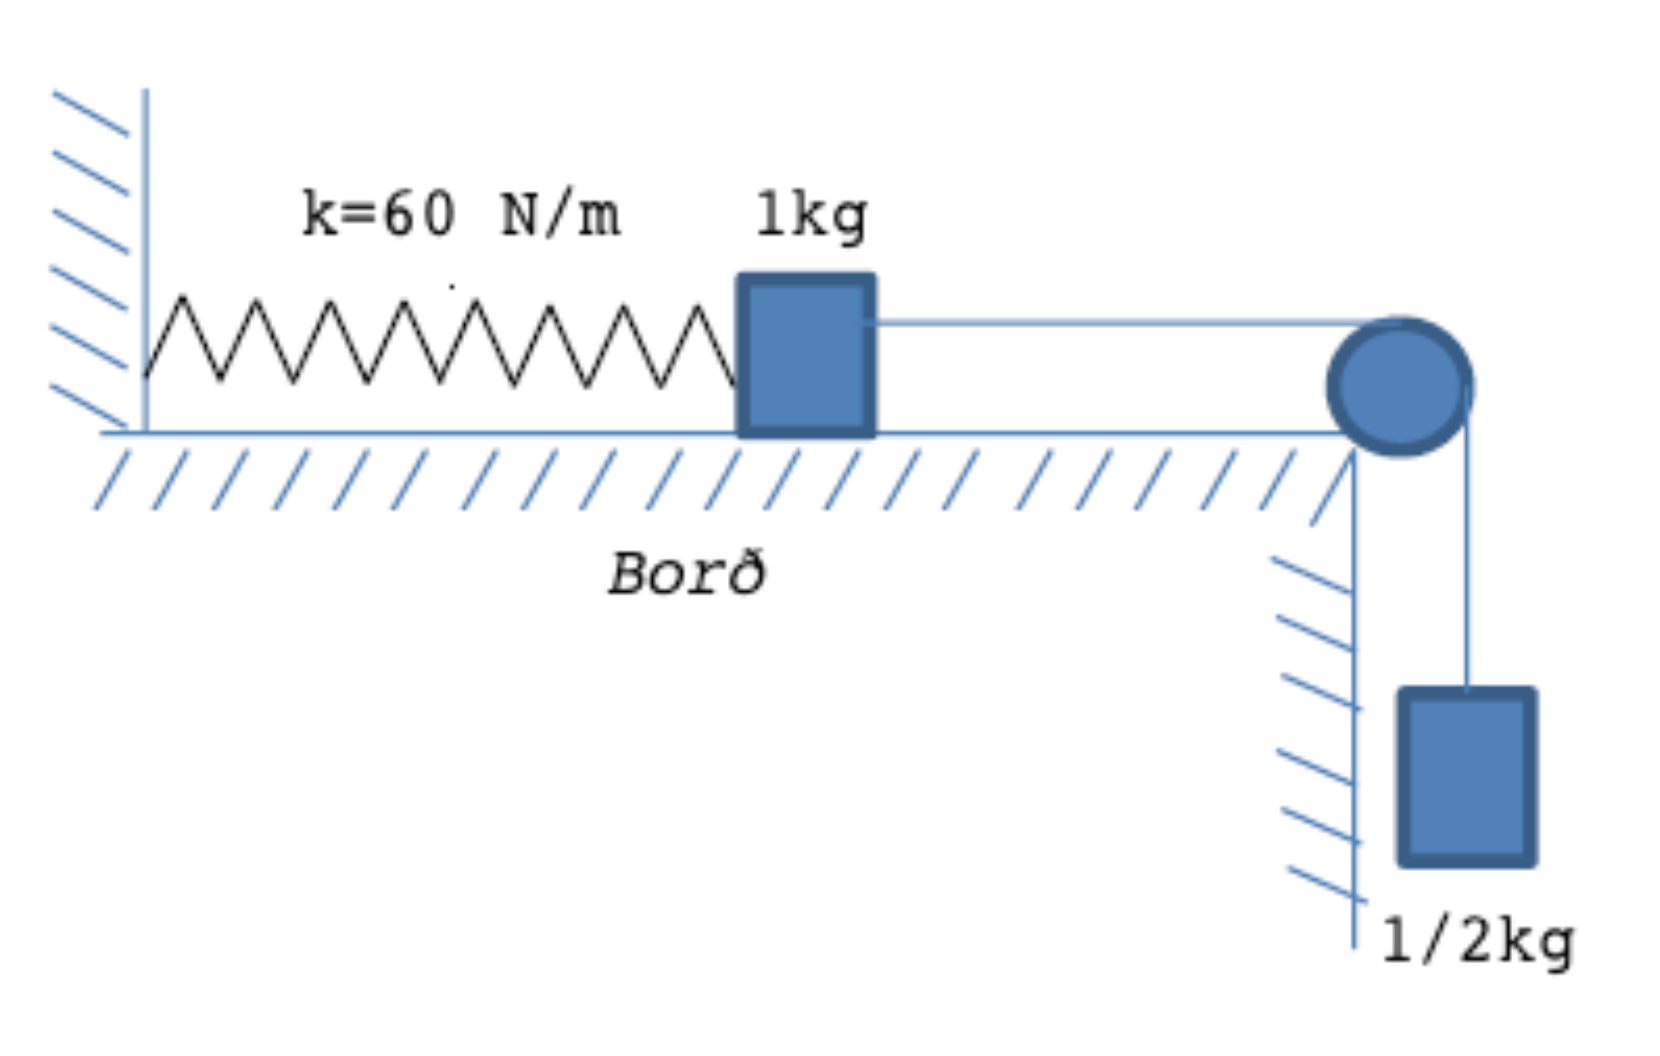
\includegraphics[width = 2in]{temp/burnspring.png}
\end{wrapfigure}

\item Lóð með massa $\SI{1.00}{kg}$ er fest í gorm með gormstuðul $k = \SI{60}{N/m}$. Lóðið er svo  tengt, með massalitlu bandi yfir núningslausa trissu í $\SI{0.50}{kg}$ massa sem hangir í bandinu. Gerum ráð fyrir að borðið sé núningslaust til einföldunar.
\begin{enumerate}[label = \textbf{(\alph*)}]
    \item Hver er strekking gormsins, $x$, frá jafnvægisstöðunni?
    
    \item Ef massalitla bandið væri brennt þannig að $\SI{0.50}{kg}$ kubburinn myndi hætta að toga í gorminn, hver yrði þá mesti hraði $\SI{1.00}{kg}$ kubbsins?
\end{enumerate}

\end{minipage}

\begin{minipage}{\linewidth}
\begin{wrapfigure}{r}{2in}
\vspace{-0.75cm}
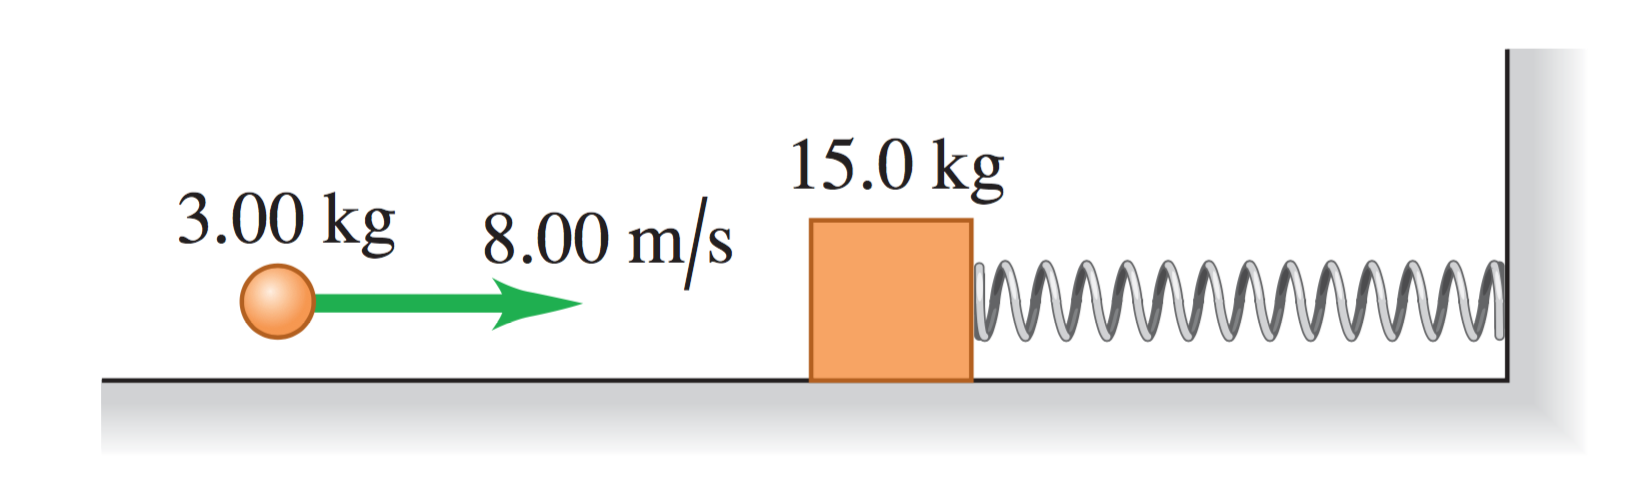
\includegraphics[scale=0.25]{temp/prob.png}
\end{wrapfigure}

\item Kyrrstæður kubbur með massa $M = \SI{15.0}{kg}$ stendur kyrr á núningslausu, láréttu borði. Kubburinn er festur við gorm, með gormstuðul $k = \SI{525}{N/m}$. Steinn með massa $m = \SI{3.00}{kg}$ og láréttan hraða $v_1 = \SI{8.00}{m/s}$ til hægri, lendir á kubbnum. Steinninn endurkastast með hraðanum $v_2 = \SI{2.00}{m/s}$ til vinstri.
\end{minipage}

\begin{enumerate}[label = \textbf{(\alph*)}]
    \item Notið skriðþungavarðveislu til þess að finna hraða kubbsins rétt eftir áreksturinn.
    \item Notið orkuvarðveislu til þess að finna mestu þjöppun gormsins eftir áreksturinn.
\end{enumerate}


\item Duge brúin nær yfir kínverska fljótið Beipan. Brúin er sú hæsta í heiminum og hefur hæðina $ h = \SI{565}{m}$ yfir vatnsborðinu. Orðrómur er um að hinn frægi frumkvöðull teygjustökksins, A.J.~Hackett, sem hefur massa $m = \SI{75}{kg}$, ætli að fara í teygjustökk fram af brúnni og freista þess að rétt svo snerta vatnsborðið. Gera má ráð fyrir að teygjan sé massalaus, af lengd $\ell = \SI{120}{m}$, og hegði sér líkt og gormur. Ekki þarf að taka tillit til hæðar Hacketts.
\begin{enumerate}[label = \textbf{(\alph*)}]
    \item Finnið gormstuðul gormsins með því að nota orkuvarðveislu.
    
    \item Hvaða hröðun mun Hackett finna fyrir þegar hann snertir vatnsborðið?
\end{enumerate}

\end{enumerate}


\section*{Svör}

\begin{enumerate*}[label = \vspace{0.15cm} \textbf{(\arabic*)}]
  \item $W_F = \SI{3200}{J}$.
  \item $F = \SI{970}{N}$, $W_F = \SI{-2800}{J}$, $W_g = \SI{4600}{J}$, $W_\mu = \SI{-1800}{J}$, $W_\text{Þ} = 0$, $W_{\text{heild}} = 0$.
  \item $v = \SI{486}{m/s}$.
  \item $x = \SI{25}{m}$.
  \item $W_F \geq \SI{1700}{kJ}$.
  \item $v_0 = \SI{95}{km/klst}$.
  \item $W = -\SI{600}{J}$, $F = \SI{3000}{N}$.
  \item $W_\mu = -\SI{630}{J}$, $\mu = 0.53$.
  \item $v = \SI{63}{m/s}$, $W_\mu = -\SI{113}{kJ}$.
  \item $v = \SI{7.7}{m/s}$, $d = \SI{0.26}{m}$.
  \item $d = \SI{53}{m}$.
  \item $v_0 = \SI{0.12}{m/s}$, $v = \SI{0.069}{m/s}$, $x = \SI{3.3}{cm}$, $\Delta K = -\SI{12}{mJ}$.
  \item $x = \SI{22}{cm}$.
  \item $d = \SI{46}{cm}$.
  \item $W_\mu = -\SI{4.0}{J}$, $\mu = 0.35$.
  \item $v = \SI{27}{m/s}$.
  \item $x = \SI{82}{mm}$, $v = \SI{0.64}{m/s}$.
  \item $u = \SI{2.0}{m/s}$, $x = \SI{34}{cm}$.
  \item $a_{\text{max}} = \SI{15.1}{m/s^2}$.
\end{enumerate*}


%%%%%%%%%%%%%%%%%%%%%%%%%%%%%%%%
%      END OF CHAPTER TEXT 
%%%%%%%%%%%%%%%%%%%%%%%%%%%%%%%%
\ifdefined \wholebook \else
 \printindex
\end{document}
\fi